%package list
\documentclass{article}
\usepackage[top=3cm, bottom=3cm, outer=3cm, inner=3cm]{geometry}
\usepackage{multicol}
\usepackage{graphicx}
\usepackage{url}
%\usepackage{cite}
\usepackage{hyperref}
\usepackage{array}
%\usepackage{multicol}
\newcolumntype{x}[1]{>{\centering\arraybackslash\hspace{0pt}}p{#1}}
\usepackage{natbib}
\usepackage{pdfpages}
\usepackage{multirow}    
\usepackage[normalem]{ulem}
\useunder{\uline}{\ul}{}
\usepackage{svg}
\usepackage{xcolor}
\usepackage{listings}
\usepackage{amsmath}
\lstdefinestyle{ascii-tree}{
    literate={├}{|}1 {─}{--}1 {└}{+}1 
  }

\lstset{basicstyle=\ttfamily,
  showstringspaces=false,
  commentstyle=\color{red},
  keywordstyle=\color{blue}
}
%\usepackage{booktabs}
\usepackage{caption}
\usepackage{subcaption}
\usepackage{float}
\usepackage{array}

\usepackage{enumitem}


\newcolumntype{M}[1]{>{\centering\arraybackslash}m{#1}}
\newcolumntype{N}{@{}m{0pt}@{}}


%%%%%%%%%%%%%%%%%%%%%%%%%%%%%%%%%%%%%%%%%%%%%%%%%%%%%%%%%%%%%%%%%%%%%%%%%%%%
%%%%%%%%%%%%%%%%%%%%%%%%%%%%%%%%%%%%%%%%%%%%%%%%%%%%%%%%%%%%%%%%%%%%%%%%%%%%
\newcommand{\itemEmail}{vmaldonadov@unsa.edu.pe}
\newcommand{\itemStudent}{Victor Gonzalo Maldonado Vilca}
\newcommand{\itemCourse}{Programación Web 2}
\newcommand{\itemCourseCode}{1702122}
\newcommand{\itemSemester}{III}
\newcommand{\itemUniversity}{Universidad Nacional de San Agustín de Arequipa}
\newcommand{\itemFaculty}{Facultad de Ingeniería de Producción y Servicios}
\newcommand{\itemDepartment}{Departamento Académico de Ingeniería de Sistemas e Informática}
\newcommand{\itemSchool}{Escuela Profesional de Ingeniería de Sistemas}
\newcommand{\itemAcademic}{2024 - A}
\newcommand{\itemInput}{Del 23 de mayo de 2024}
\newcommand{\itemOutput}{Al 24 de junio de 2024}
\newcommand{\itemPracticeNumber}{08}
\newcommand{\itemTheme}{Django 4}
%%%%%%%%%%%%%%%%%%%%%%%%%%%%%%%%%%%%%%%%%%%%%%%%%%%%%%%%%%%%%%%%%%%%%%%%%%%%
%%%%%%%%%%%%%%%%%%%%%%%%%%%%%%%%%%%%%%%%%%%%%%%%%%%%%%%%%%%%%%%%%%%%%%%%%%%%

\usepackage[english,spanish]{babel}
\usepackage[utf8]{inputenc}
\AtBeginDocument{\selectlanguage{spanish}}
\renewcommand{\figurename}{Figura}
\renewcommand{\refname}{Referencias}
\renewcommand{\tablename}{Tabla} %esto no funciona cuando se usa babel
\AtBeginDocument{%
	\renewcommand\tablename{Tabla}
}

\usepackage{fancyhdr}
\pagestyle{fancy}
\fancyhf{}
\setlength{\headheight}{30pt}
\renewcommand{\headrulewidth}{1pt}
\renewcommand{\footrulewidth}{1pt}
\fancyhead[L]{\raisebox{-0.2\height}{
\includegraphics[width=3cm]{img/logo_episunsa.png}}}
\fancyhead[C]{\fontsize{7}{7}\selectfont	\itemUniversity \\ \itemFaculty \\ \itemDepartment \\ \itemSchool \\ \textbf{\itemCourse}}
\fancyhead[R]{\raisebox{-0.2\height}{
\includegraphics[width=1.2cm]{img/logo_abet}}}
\fancyfoot[L]{Victor M.}
\fancyfoot[C]{\itemCourse}
\fancyfoot[R]{Página \thepage}

% para el codigo fuente
\usepackage{listings}
\usepackage{color, colortbl}
\definecolor{dkgreen}{rgb}{0,0.6,0}
\definecolor{gray}{rgb}{0.5,0.5,0.5}
\definecolor{mauve}{rgb}{0.58,0,0.82}
\definecolor{codebackground}{rgb}{0.95, 0.95, 0.92}
\definecolor{tablebackground}{rgb}{0.8, 0, 0}
\definecolor{gitgreen}{RGB}{40, 160, 40}
\definecolor{gitred}{RGB}{255, 0, 0}
\definecolor{gitgray}{RGB}{128, 128, 128}

\lstset{frame=tb,
	language=bash,
	aboveskip=3mm,
	belowskip=3mm,
	showstringspaces=false,
	columns=flexible,
	basicstyle={\small\ttfamily},
	numbers=none,
	numberstyle=\tiny\color{gray},
	keywordstyle=\color{blue},
	commentstyle=\color{dkgreen},
	stringstyle=\color{mauve},
	breaklines=true,
	breakatwhitespace=true,
	tabsize=3,
	backgroundcolor= \color{codebackground},
}

\begin{document}
	
	\vspace*{10px}
	
	\begin{center}	
		\fontsize{17}{17} \textbf{ Informe de Django 04}
	\end{center}
	\centerline{\textbf{\Large Tema: \itemTheme}}
	%\vspace*{0.5cm}	

	\begin{flushright}
		\begin{tabular}{|M{2.5cm}|N|}
			\hline 
			\rowcolor{tablebackground}
			\color{white} \textbf{Nota}  \\
			\hline 
			     \\[30pt]
			\hline 			
		\end{tabular}
	\end{flushright}	

	\begin{table}[H]
		\begin{tabular}{|x{4.7cm}|x{4.8cm}|x{4.8cm}|}
			\hline 
			\rowcolor{tablebackground}
			\color{white} \textbf{Estudiante} & \color{white}\textbf{Escuela}  & \color{white}\textbf{Asignatura}   \\
			\hline 
			{\itemStudent \par \itemEmail} & \itemSchool & {\itemCourse \par Semestre: \itemSemester \par Código: \itemCourseCode}     \\
			\hline 			
		\end{tabular}
	\end{table}		
	
	\begin{table}[H]
		\begin{tabular}{|x{4.7cm}|x{4.8cm}|x{4.8cm}|}
			\hline 
			\rowcolor{tablebackground}
			\color{white}\textbf{Tarea} & \color{white}\textbf{Tema}  & \color{white}\textbf{Duración}   \\
			\hline 
			\itemPracticeNumber & \itemTheme & 2 horas   \\
			\hline 
		\end{tabular}
	\end{table}
	
	\begin{table}[H]
		\begin{tabular}{|x{4.7cm}|x{4.8cm}|x{4.8cm}|}
			\hline 
			\rowcolor{tablebackground}
			\color{white}\textbf{Semestre académico} & \color{white}\textbf{Fecha de inicio}  & \color{white}\textbf{Fecha de entrega}   \\
			\hline 
			\itemAcademic & \itemInput &  \itemOutput  \\
			\hline 
		\end{tabular}
	\end{table}
  
%%%%%%%%%%%%%%%%%%%%
 
	\section{Tarea}
  \begin{itemize}
    \item Repetir las actividades vistas en teoria de Django4.  Ir haciendo commits cada avance.  Compartirlo con el docente (CarloCorrales010)
  \end{itemize}
  
%%%%%%%%%%%%%%%%%%%% 
 
  \section{Entregables}
  \begin{itemize}
    \item Informe hecho en Latex.
    \item \textbf{texto: }Respuestas a las preguntas de las diapositivas 
    \item Captura de pantalla del siguiente comando:
    \begin{lstlisting}[language=bash]
      git log --graph --pretty=oneline --abbrev-commit --all
    \end{lstlisting}
    \item URL - Repositorio GitHub
  \end{itemize}
  
%%%%%%%%%%%%%%%%%%%%    
		
	\section{Equipos, materiales y temas utilizados}
  \begin{itemize}
    \item Configuración de Proyectos
    \item Modelado de Datos
    \item Migraciones de Base de Datos
    \item Desarrollo de Vistas y URLs
    \item Uso de Plantillas HTML
    \item Administración de Aplicaciones
    \item Control de Versiones
    \item Creacion y manejo de Formularios
  \end{itemize}

%%%%%%%%%%%%%%%%%%%%

	\section{Respuestas a las Preguntas dejadas en las Diapositivas}
  \begin{enumerate}
    \item \textbf{¿El formulario tiene los mismos campos y tipos que el modelo?}
      \newline
      \textbf{Respuesta: }Sí,debido a que en el formulario se integran los mismos campos y tipos de datos que encontramos en el modelo, 
      es cierto que estos formularios ya no heredan de un modelo en particular, pero cumple con los campos ya establecidos en el modelo 
      permitiendo ue el formulario capture y valide datos de acuerdo con la estructura definida en el modelo, aunque no esté vinculado de manera directa.
    \item \textbf{¿Cuál es el valor para las opciones core by default?}
      \newline
      \textbf{Respuesta: }Los valores por defecto de las opciones core son: 
      \begin{itemize}
        \item \textbf{required = True}: Se refiere a que el campo debe ser llenado obligatoriamente por el usuario; es otras palabras, 
        no puede quedar vacío.
        \item \textbf{widget=None}: Se refiere a que el campo utilizará el widget estándar adecuado para su tipo de datos, siendo seleccionado 
        automáticamente si no se especifica.
        \item \textbf{label=None}: Se refiere que el campo no tendrá una etiqueta predeterminada; en caso de ser None, se generará una etiqueta 
        basada en el nombre del campo.
        \item \textbf{initial=None}: Representa el valor inicial por defecto para el campo; si se omite, el campo estará vacío inicialmente.
        \item \textbf{\text{help\_text}=''}: Significa que se puede proporcionar un texto de ayuda opcional para el campo; si se deja vacío, no se mostrará ninguna ayuda.
      \end{itemize}
  \end{enumerate}

%%%%%%%%%%%%%%%%%%%%

	\section{Captura de Pantalla}
  \begin{figure}[H]
    \centering
    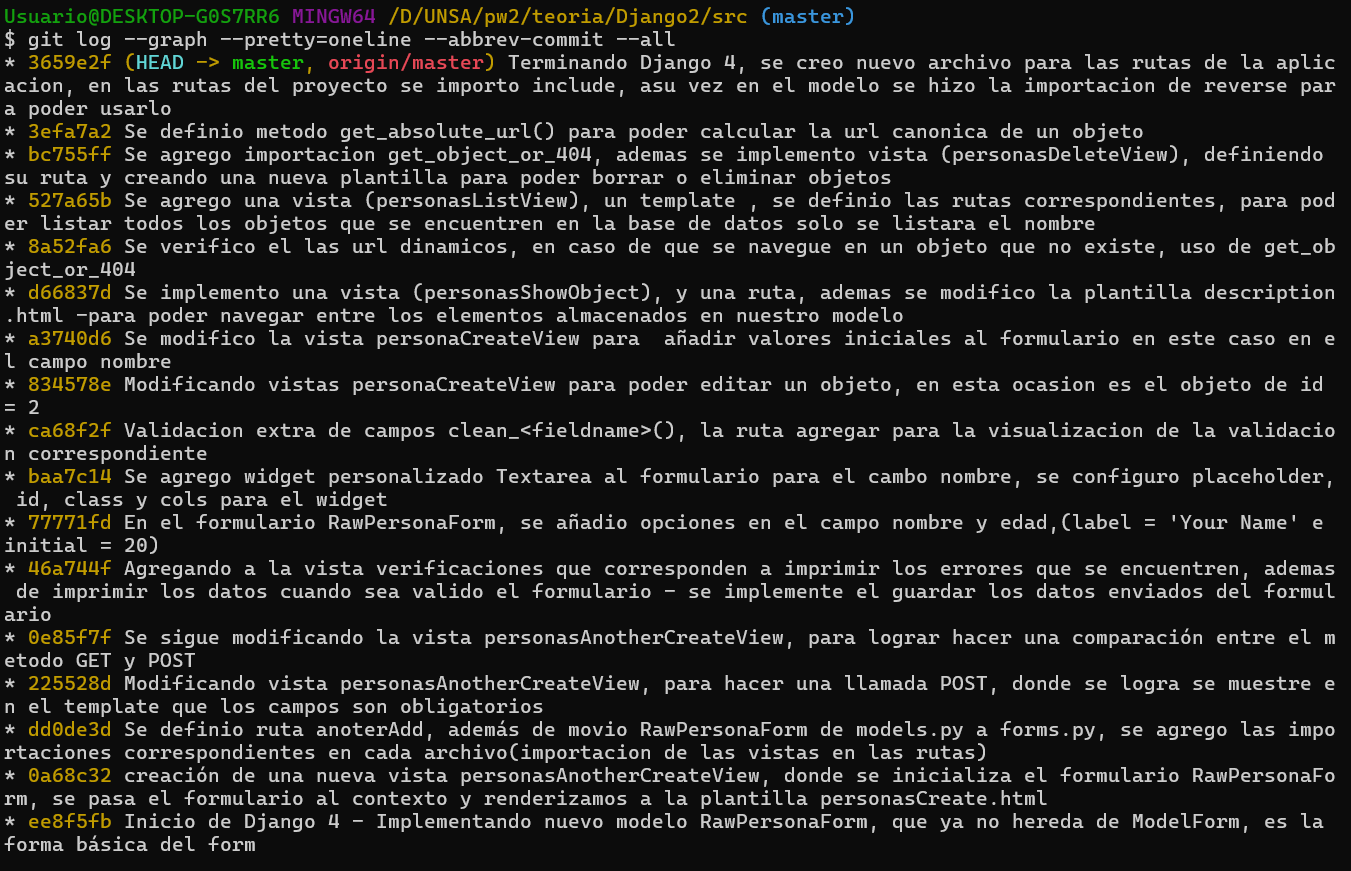
\includegraphics[width=1\textwidth, keepaspectratio]{img/commits1.png}
    \caption{commits - local}
  \end{figure}

%%%%%%%%%%%%%%%%%%%%

  \section{URL de Repositorio Github}
  \begin{itemize}
    \item URL del Repositorio GitHub.
    \item \url{https://github.com/Victor-Gonzalo-Maldonado-Vilca/Django2.git}
  \end{itemize}

%%%%%%%%%%%%%%%%%%%%

  \section{Desarrollo del trabajo}
  \textit{Continuamos a partir del proyecto realizado en Django 3}
  
%%%%%%%%%%%%

  \subsection{Imágenes de Ejecución}
  \begin{figure}[H]
    \centering
    \fbox{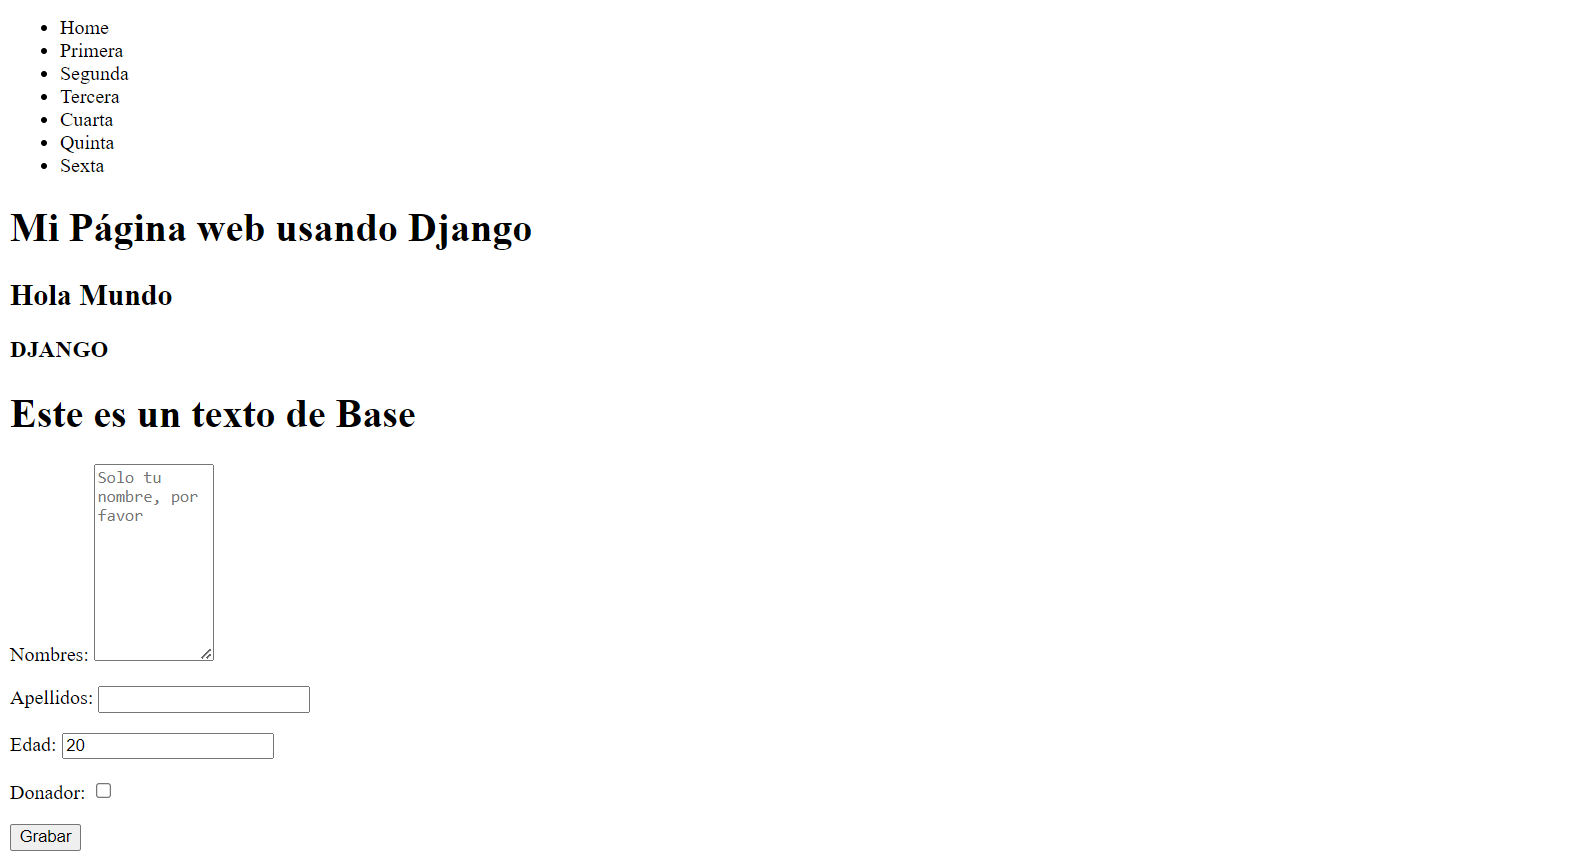
\includegraphics[width=1\textwidth, keepaspectratio]{img/ejecucion0.png}}
    \caption{Agregar Objetos}
  \end{figure}
  \begin{figure}[H]
    \centering
    \fbox{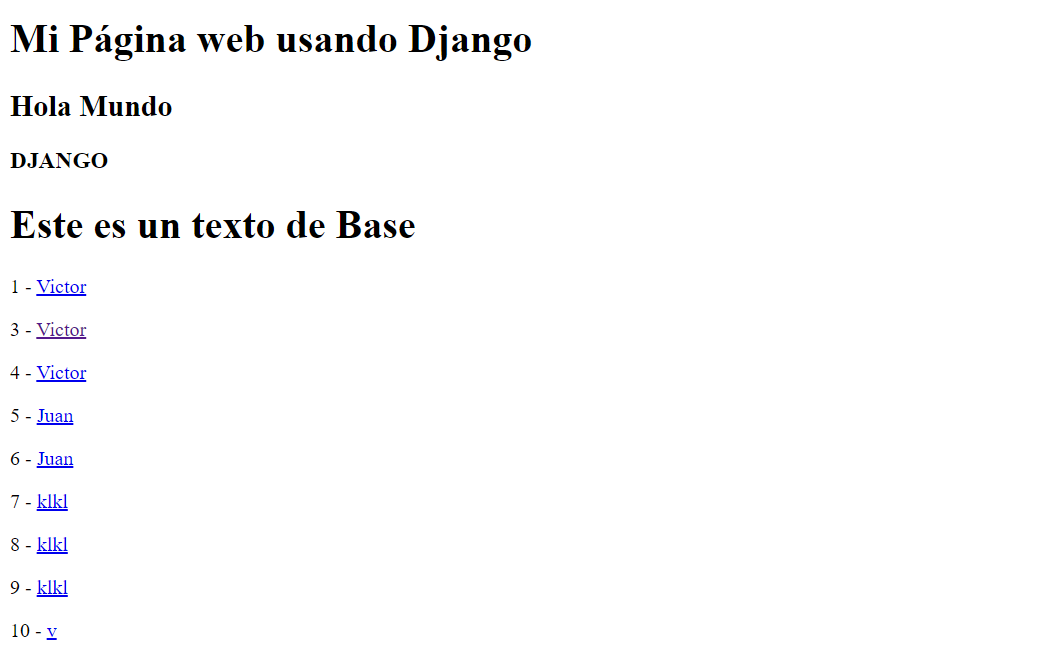
\includegraphics[width=1\textwidth, keepaspectratio]{img/ejecucion1.png}}
    \caption{Listar objetos}
  \end{figure}
  \begin{figure}[H]
    \centering
    \fbox{
\includegraphics[width=1\textwidth, keepaspectratio]{img/ejecucion2.png}}
    \caption{Visualizar Objetos Especificos}
  \end{figure}
  \begin{figure}[H]
    \centering
    \fbox{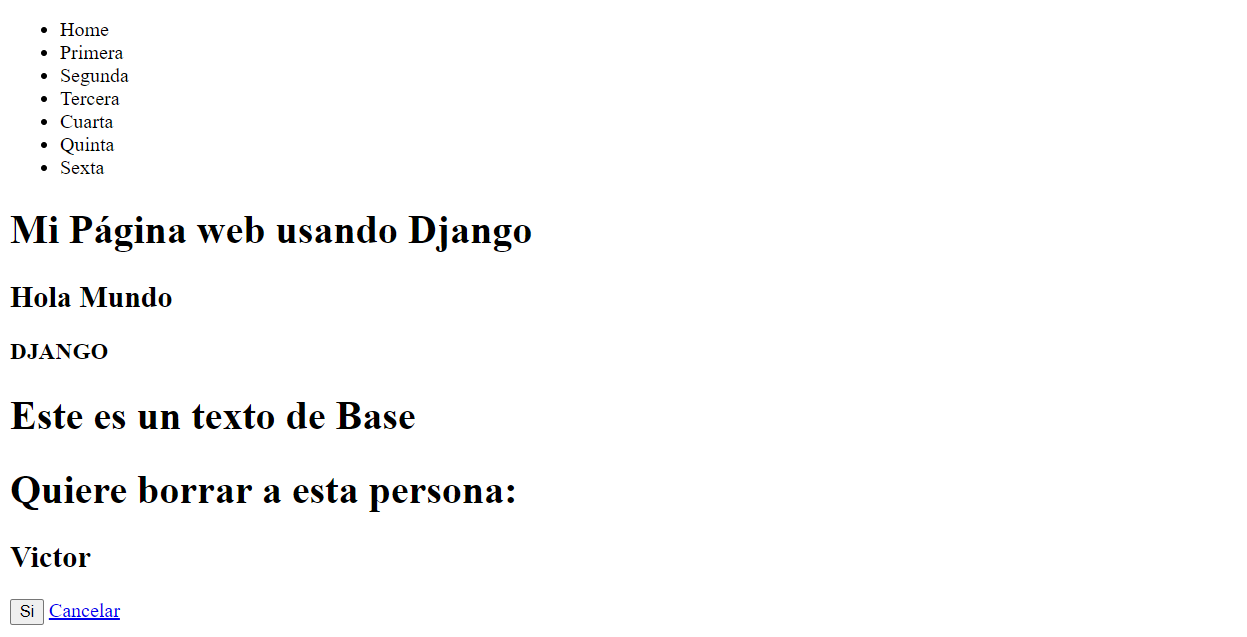
\includegraphics[width=1\textwidth, keepaspectratio]{img/ejecucion3.png}}
    \caption{Eliminar objetos}
  \end{figure}
  
%%%%%%%%%%%%

  \subsection{Modelos -- Aplicación personas}
  Se definio la función $\text{get\_absolute\_url}$ en Django se utiliza para obtener la URL absoluta de una instancia de un modelo específico. 
  En el siguiente código, la función devuelve la URL que apunta a la vista 'personas:browsing' con el parámetro myID igual al id de la 
  instancia actual.
  \begin{lstlisting}[language=Python, caption={Modelo Persona}]
    def get_absolute_url(self):
      return reverse('personas:browsing', kwargs={'myID': self.id})
  \end{lstlisting}
    
%%%%%%%%%%%%

  \subsection{Vistas -- Aplicación personas}
  
%%%%%%
  
  \subsubsection{Vista personasAnotherCreateView()}
  \begin{itemize}
    \item \textbf{Descripción: }Se define una vista llamada personasAnotherCreateView, diseñada para gestionar la creación de instancias de 
    objetos Persona utilizando un formulario personalizado denominado RawPersonaForm.
    \newline
    Primero, se inicializa el formulario RawPersonaForm para recopilar los datos necesarios para crear una nueva persona. Luego, 
    se verifica si la solicitud es de tipo POST. En caso afirmativo, se intenta procesar el formulario con los datos recibidos.
    \newline
    Si el formulario es válido según la función $\text{is\_valid()}$, se imprimen los datos limpios $\text{(cleaned\_data)}$ del formulario para su revisión 
    y se procede a crear una nueva instancia de Persona utilizando estos datos validados. En caso de que el formulario no sea válido, se 
    imprimen los errores generados por el formulario para su corrección.
    \newline
    Finalmente, se prepara el contexto con el formulario y cualquier otra información necesaria, y se renderiza la plantilla 
    'personas/personasCreate.html' para que el usuario pueda interactuar con el formulario de creación de personas.
    \item \textbf{Código: }
    \begin{lstlisting}[language=Python]
      def personasAnotherCreateView(request):
        form = RawPersonaForm()
        if request.method == "POST":
            form = RawPersonaForm(request.POST)
            if form.is_valid():
                print(form.cleaned_data)
                Persona.objects.create(**form.cleaned_data)
            else:
                print(form.errors)
        context = {
            'form': form,
        }
        return render(request, 'personas/personasCreate.html', context)
  \end{lstlisting}   
  \end{itemize}
  
%%%%%%
  
  \subsubsection{Vista personasShowObject()}
  \begin{itemize}
    \item \textbf{Descripción: }La presente vista se encarga de mostrar los detalles de una instancia específica de Persona según el 
    ID proporcionado en la solicitud. Primero, se utiliza $\text{get\_object\_or\_404}$ para obtener la instancia de Persona correspondiente al 
    ID especificado. Si no se encuentra ninguna instancia con ese ID, se muestra una página 404.
    \newline
    Luego, se prepara el contexto con el objeto obj y se renderiza la plantilla 'personas/description.html', que probablemente contenga 
    la estructura HTML para mostrar la información detallada de la persona en el frontend.
    \item \textbf{Código: }
    \begin{lstlisting}[language=Python]
      def personasShowObject(request, myID):
        obj = get_object_or_404(Persona, id = myID)
        context = {
            'objeto': obj,
        }
        return render(request, 'personas/description.html', context)
    \end{lstlisting}   
  \end{itemize}
  
%%%%%%
  
  \subsubsection{Vista personasListView()}
  \begin{itemize}
    \item \textbf{Descripción: }Esta vista obtiene todos los objetos Persona de la base de datos utilizando `Persona.objects.all()`.
    Luego, prepara el contexto con la lista de objetos Persona y renderiza la plantilla 'personas/personasLista.html', 
    que probablemente contenga la estructura HTML para mostrar la lista de personas en el frontend de la aplicación.
    \item \textbf{Código: }
    \begin{lstlisting}[language=Python]
      def personasListView(request):
        queryset = Persona.objects.all()
        context = {
            'objectList': queryset,
        }
        return render(request, 'personas/personasLista.html', context)
    \end{lstlisting}   
  \end{itemize}
  
%%%%%%
  
  \subsubsection{Vista personasDeleteView()}
  \begin{itemize}
    \item \textbf{Descripción: }Esta vista elimina una instancia específica de Persona según el ID proporcionado en la solicitud POST. 
    Primero, se obtiene la instancia de Persona o se muestra una página 404 si no se encuentra. Luego, si la solicitud es POST, se elimina 
    la instancia y se redirige al usuario a la página principal. En caso contrario, se muestra un formulario de confirmación en la plantilla 
    `'personas/personasBorrar.html'`.
    \item \textbf{Código: }
    \begin{lstlisting}[language=Python]
      def personasDeleteView(request, myID):
        obj = get_object_or_404(Persona, id = myID)
        if request.method == 'POST':
            print("lo borro")
            obj.delete()
            return redirect('../')
        context = {
            'objeto': obj,
        }
        return render(request, 'personas/personasBorrar.html', context)
    \end{lstlisting}   
  \end{itemize}
  
%%%%%%%%%%%%

  \subsection{Formularios - Apicación personas}
  
%%%%%%
  
  \subsubsection{Formulario PersonaForm()}
  \begin{itemize}
    \item \textbf{Descripción: }Se define el método $\text{clean\_nombres}$ que verifica si el valor ingresado en el campo 'nombre' tiene 
    la primera letra en mayúscula. Si es así, el método devuelve el nombre sin realizar ninguna modificación. En caso contrario, 
    se lanza una excepción ValidationError con el mensaje 'La primera letra en Mayuscula'.
    \newpage
    \item \textbf{Código: }
    \begin{lstlisting}[language=Python]
      def clean_nombres(self, *args, **kwargs):
        print('paso')
        name = self.cleaned_data.get('nombre')
        if name.istitle():
            return name
        else:
            raise forms.ValidationError('La primera letra en Mayuscula')
    \end{lstlisting}   
  \end{itemize}
  
%%%%%%
  
  \subsubsection{Formulario RawPersonaForm()}
  \begin{itemize}
    \item \textbf{Descripción: }El formulario RawPersonaForm se utiliza para recopilar información sobre una persona. 
    Incluye campos para el nombre, apellidos, edad y la opción de indicar si la persona es donadora. El campo de nombres utiliza un 
    widget de Textarea con características adicionales como marcador de posición, identificador, clase y número de columnas. 
    El campo de edad tiene un valor inicial predeterminado de 20 años. Este formulario proporciona una interfaz sencilla para 
    que los usuarios ingresen información básica sobre una persona.
    \item \textbf{Código: }
    \begin{lstlisting}[language=Python]
      class RawPersonaForm(forms.Form):
        nombres   = forms.CharField(
            widget = forms.Textarea(
                attrs={
                    'placeholder': 'Solo tu nombre, por favor',
                    'id': 'nombreID',
                    'class': 'special',
                    'cols': 10,
                }
            )
        )
        apellidos = forms.CharField()
        edad      = forms.IntegerField(initial = 20)
        donador   = forms.BooleanField()
    \end{lstlisting}   
  \end{itemize}
  
%%%%%%%%%%%%

  \subsection{URLs}
  
%%%%%%
  
  \subsubsection{urls del proyecto listaContactos}
  \begin{itemize}
    \item \textbf{Descripción: }El archivo urls.py importa las funciones necesarias para manejar las rutas URL, como path y include, 
    junto con las vistas myHomeView y anotherView desde el módulo views de la aplicación inicio. Las rutas URL se configuran de la 
    siguiente manera: la ruta 'personas/' incluye las URLs de la aplicación personas, la ruta 'admin/' está asignada a la interfaz 
    de administración de Django, la ruta raíz ('') dirige a la vista myHomeView con el nombre 'Página de Inicio', y la ruta 'another/' 
    se relaciona con la vista anotherView y se le asigna el nombre 'otro'.
    \item \textbf{Código: }
    \begin{lstlisting}[language=Python]
      from django.contrib import admin
      from django.urls import path, include
      from inicio.views import myHomeView, anotherView

      urlpatterns = [
          path('personas/', include('personas.urls')),
          path('admin/', admin.site.urls),
          path('', myHomeView, name='Pagina de Inicio'),
          path('another/', anotherView, name='otro'),
      ]
    \end{lstlisting}   
  \end{itemize}
  
%%%%%%
  
  \subsubsection{urls de la aplicación personas}
  \begin{itemize}
    \item \textbf{Descripción: }El archivo urls.py maneja las rutas URL relacionadas con las vistas de personas. 
    Incluye rutas como `'persona/'` para personaTestView, 'agregar/' para personaCreateView, `'personas/<int:myID>/'` 
    para personasShowObject, la ruta raíz ('') para personasListView, y `'personas/<int:myID>/delete'` para personasDeleteView.
    \item \textbf{Código: }
    \begin{lstlisting}[language=Python]
      from django.urls import path
      from personas.views import personasDeleteView, personasListView, personaTestView, personaCreateView, searchForHelp,  personasAnotherCreateView, personasShowObject

      app_name = 'personas'
      urlpatterns = [
          path('persona/', personaTestView, name='testViewPersona'),
          path('agregar/', personaCreateView, name='createPersona'),
          path('personas/<int:myID>/', personasShowObject, name = 'browsing'),
          path('', personasListView, name = 'listing'),
          path('personas/<int:myID>/delete', personasDeleteView, name = 'deleting'),
      ]
    \end{lstlisting}   
  \end{itemize}

%%%%%%%%%%%%%%%%%%%%%

  \section{Templates}
  \textit{En esta actividad se realizo 2 templates}
  
%%%%%%%%%%%%

  \subsection{Plantilla personasLista.html}
  \begin{itemize}
    \item \textbf{Descripción: } Se define una estructura HTML básica con metadatos y un título. Luego, extiende el contenido del archivo base.html utilizando la directiva 
     extends 'base.html' . Dentro del bloque de contenido block content , utiliza un bucle for para iterar sobre cada 
    instancia en la lista de objetos (objectList). Para cada instancia, muestra su ID y nombre como un enlace. Al hacer clic en el nombre, 
    se redirige a la URL absoluta definida en el método $\text{get\_absolute\_url}$ de la instancia.
    \item \textbf{Código: }
    \begin{lstlisting}[language=html]
      <!DOCTYPE HTML>
      <html>
        <head>
          <meta charset="UTF-8"/>
          <meta name="viewport" content="width=device-width, initial-scale=1.0"/>
          <title>test</title>
        </head>
        <body>
          
          
          
            <p> {{instance.id}} 
            - 
              <a href='{{instance.get_absolute_url}}'>
                {{instance.nombre}}
              </a>
            </p>
          
          
        </body>
      </html>
    \end{lstlisting}
  \end{itemize}
  
%%%%%%%%%%%%

  \subsection{Plantilla personasBorrar.html}
  \begin{itemize}
    \item \textbf{Descripción: }En este template se define un formulario que se envía utilizando el método POST y contiene un token CSRF para protección contra ataques 
    de falsificación de solicitudes entre sitios. En el formulario, se muestra el nombre de la persona que se va a eliminar `({{objeto.nombre}})`
    junto con un mensaje preguntando si se desea borrar a esa persona. Se incluyen dos opciones para el usuario: un botón de enviar ('Si') 
    para confirmar la eliminación y un enlace para cancelar la acción y regresar a la página anterior.
    \item \textbf{Código: }
    \begin{lstlisting}[language=html]
      <!DOCTYPE HTML>
      <html>
        <head>
          <meta charset="UTF-8"/>
          <meta name="viewport" content="width=device-width, initial-scale=1.0"/>
          <title>test</title>
        </head>
        <body>
          
          
          <form method='POST'> 
            <h1>Quiere borrar a esta persona: </h1>
            <h2>{{objeto.nombre}}</h2>
            <input type='submit' value='Si'/>
            <a href='../'>Cancelar</a>
          </form>
          
        </body>
      </html>
    \end{lstlisting}
  \end{itemize}
  
%%%%%%%%%%%%

  \subsection{Ejecución del servidor}
  Este siguiente comando inicia el servidor local de Django. Una vez ejecutado, el servidor estará disponible por defecto en la dirección 
  \texttt{http://127.0.0.1:8000/}. Desde esta dirección, se puede acceder a las diferentes vistas y funcionalidades del 
  proyecto Django.
  \begin{lstlisting}[language=bash]
    python manage.py runserver
  \end{lstlisting}

%%%%%%%%%%%%%%%%%%%%

  \section{Conclusiones}
  \begin{itemize}
    \item El aprendizaje sobre el desarrollo en Django ha sido significativo, abarcando aspectos clave como 
    la configuración de rutas URL, definición de vistas y creación de formularios.
    \item La comprensión de la estructura de proyectos en Django, incluyendo la organización de aplicaciones, modelos y 
    archivos de configuración, es esencial para un desarrollo eficiente.
    \item La utilización de herramientas como el servidor de desarrollo de Django y el sistema de plantillas facilitaron 
    el desarrollo ágil y eficiente de la aplicación.
    \item Django es un framework web potente y versátil que permite desarrollar aplicaciones web de manera rápida y eficiente.
    \item La arquitectura MVC (Modelo-Vista-Controlador) de Django ayuda a organizar el código de manera estructurada y modular, 
    lo que facilita la mantenibilidad y escalabilidad de las aplicaciones.
    \item Con un buen entendimiento de Django y siguiendo las mejores prácticas de desarrollo, se pueden crear aplicaciones web 
    robustas y de alto rendimiento.
  \end{itemize}
  
%%%%%%%%%%%%%%%%%%%%
	\newpage
	\subsection{\textcolor{red}{Rúbrica para el contenido del Informe y demostración}}
	\begin{itemize}			
		\item El alumno debe marcar o dejar en blanco en celdas de la columna \textbf{Checklist} si cumplio con el ítem correspondiente.
		\item Si un alumno supera la fecha de entrega,  su calificación será sobre la nota mínima aprobada, siempre y cuando cumpla con todos lo items.
		\item El alumno debe autocalificarse en la columna \textbf{Estudiante} de acuerdo a la siguiente tabla:
	
		\begin{table}[ht]
			\caption{Niveles de desempeño}
			\begin{center}
			\begin{tabular}{ccccc}
    			\hline
    			 & \multicolumn{4}{c}{Nivel}\\
    			\cline{1-5}
    			\textbf{Puntos} & Insatisfactorio 25\%& En Proceso 50\% & Satisfactorio 75\% & Sobresaliente 100\%\\
    			\textbf{2.0}&0.5&1.0&1.5&2.0\\
    			\textbf{4.0}&1.0&2.0&3.0&4.0\\
    		\hline
			\end{tabular}
		\end{center}
	\end{table}	
	

	\end{itemize}

 
	
	\begin{table}[H]
		\caption{Rúbrica para contenido del Informe y demostración}
		\setlength{\tabcolsep}{0.5em} % for the horizontal padding
		{\renewcommand{\arraystretch}{1.5}% for the vertical padding
		%\begin{center}
		\begin{tabular}{|p{2.7cm}|p{7cm}|x{1.3cm}|p{1.2cm}|p{1.5cm}|p{1.1cm}|}
			\hline
    		\multicolumn{2}{|c|}{Contenido y demostración} & Puntos & Checklist & Estudiante & Profesor\\
			\hline
			\textbf{1. GitHub} & Hay enlace URL activo del directorio para el  laboratorio hacia su repositorio GitHub con código fuente terminado y fácil de revisar. &2 &X &2 & \\ 
			\hline
			\textbf{2. Commits} &  Hay capturas de pantalla de los commits más importantes con sus explicaciones detalladas. (El profesor puede preguntar para refrendar calificación). &4 &X &4 & \\ 
			\hline 
			\textbf{3. Código fuente} &  Hay porciones de código fuente importantes con numeración y explicaciones detalladas de sus funciones. &2 &X &2 & \\ 
			\hline 
			\textbf{4. Ejecución} & Se incluyen ejecuciones/pruebas del código fuente  explicadas gradualmente. &2 &X &2 & \\ 
			\hline			
			\textbf{5. Pregunta} & Se responde con completitud a la pregunta formulada en la tarea.  (El profesor puede preguntar para refrendar calificación).  &2 &X &2 & \\ 
			\hline	
			\textbf{6. Fechas} & Las fechas de modificación del código fuente estan dentro de los plazos de fecha de entrega establecidos. &2 &X &2 & \\ 
			\hline 
			\textbf{7. Ortografía} & El documento no muestra errores ortográficos. &2 &X &2 & \\ 
			\hline 
			\textbf{8. Madurez} & El Informe muestra de manera general una evolución de la madurez del código fuente,  explicaciones puntuales pero precisas y un acabado impecable.   (El profesor puede preguntar para refrendar calificación).  &4 &X &4 & \\ 
			\hline
			\multicolumn{2}{|c|}{\textbf{Total}} &20 & &20 & \\ 
			\hline
		\end{tabular}
		%\end{center}
		%\label{tab:multicol}
		}
	\end{table}


%%%%%%%%%%%%%%%%%%%%%%%%%%%%%%%%%%%%%%%%%%%%%%%%%%%%%%%%%%%%%%%%%%%
	
  \newpage
  \section{Referencias}
  \begin{itemize}
    \item \url{https://docs.djangoproject.com/en/5.0/}
    \item \url{https://docs.github.com/es}
    \item \url{https://git-scm.com/doc}
  \end{itemize}
  
%%%%%%%%%%%%%%%%%%%% 
%\clearpage
%\bibliographystyle{apalike}
%\bibliographystyle{IEEEtranN}
%\bibliography{bibliography}
			
\end{document}
